%
% Clases de módulo de FFX.
% Análisis y diseño de programa tokenizador, reporte técnico.
%
% Proyecto Lovelace.
%

\subsection{Clases de \texorpdfstring{\acrshort{gl:ffx}}{FFX}}

En la figura~\ref{clases_ffx} se muestran las clases que conforman al módulo de
FFX. Sin contar a las tres interfaces de funciones (que forman parte del paquete
de utilidades) todas las clases son del paquete de implementaciones.

La clase de la red Feistel implementa la interfaz de una función con inverso
(tiene tanto operación de ida, como de vuelta) y se compone (por medio de una
relación de composición) de una función, utilizada como función de ronda, y de
una función con inverso, utilizada como operador de combinación. Ambas clases
hijas (redes Feistel alternantes o desbalanceadas) contienen un indicador de
desbalanceo y sobreescriben ambas operaciones de la superclase; la red feistel
alternante (ver sección~\ref{sec:red_feistel}) agrega una nueva función
de ronda: una para las pares y otra para las impares.

En la parte superior de diagrama se muestran las dos posibles operaciones de
combinación que soporta ffx: una a nivel de bloque y la otra nivel de caracter.
La única clase en donde estas dos opciones son reestrictivas es desde la
construcción de FFXA10; el desacoplamiento dado por las interfaces permite que
lo único que necesite saber la red es que tiene una función que recibe un
arreglo y entrega un arreglo.

Otra clase con la misma esructura que las dos anteriores es la de la función de
ronda de FFXA10: implementa la interfaz de una función con inverso simétrico
(que a su vez implementa un función con inverso); una instancia de esta clase
en FFX es usada para construir a la red Feistel con la que se opera.

La clase de FFX es solamente un medio de comunicación con la red Feistel
interna, esto es, no agrega ninguna lógica extra a los procesos de operación y
operación inversa. Lo mismo ocurre con FFXA10; solo que mientras el contructor
de la superclase es abierto a personalizar la red (FFX debería servir para
cualquier cifrado que preserva el formato, no solo para un alfabeto de
dígitos), el contructor de FFXA10 tiene parámetros bastante limitados, y su
construcción de la superclase y la red Feistel ya es predefinida según la
descripción de esta colección hecha en la sección~\ref{sec:ffx}. Es esta última
clase (FFXA10) la que implementa la interfaz de los algoritmos tokenizadores
reversibles.

\begin{sidewaysfigure}
  \begin{center}
    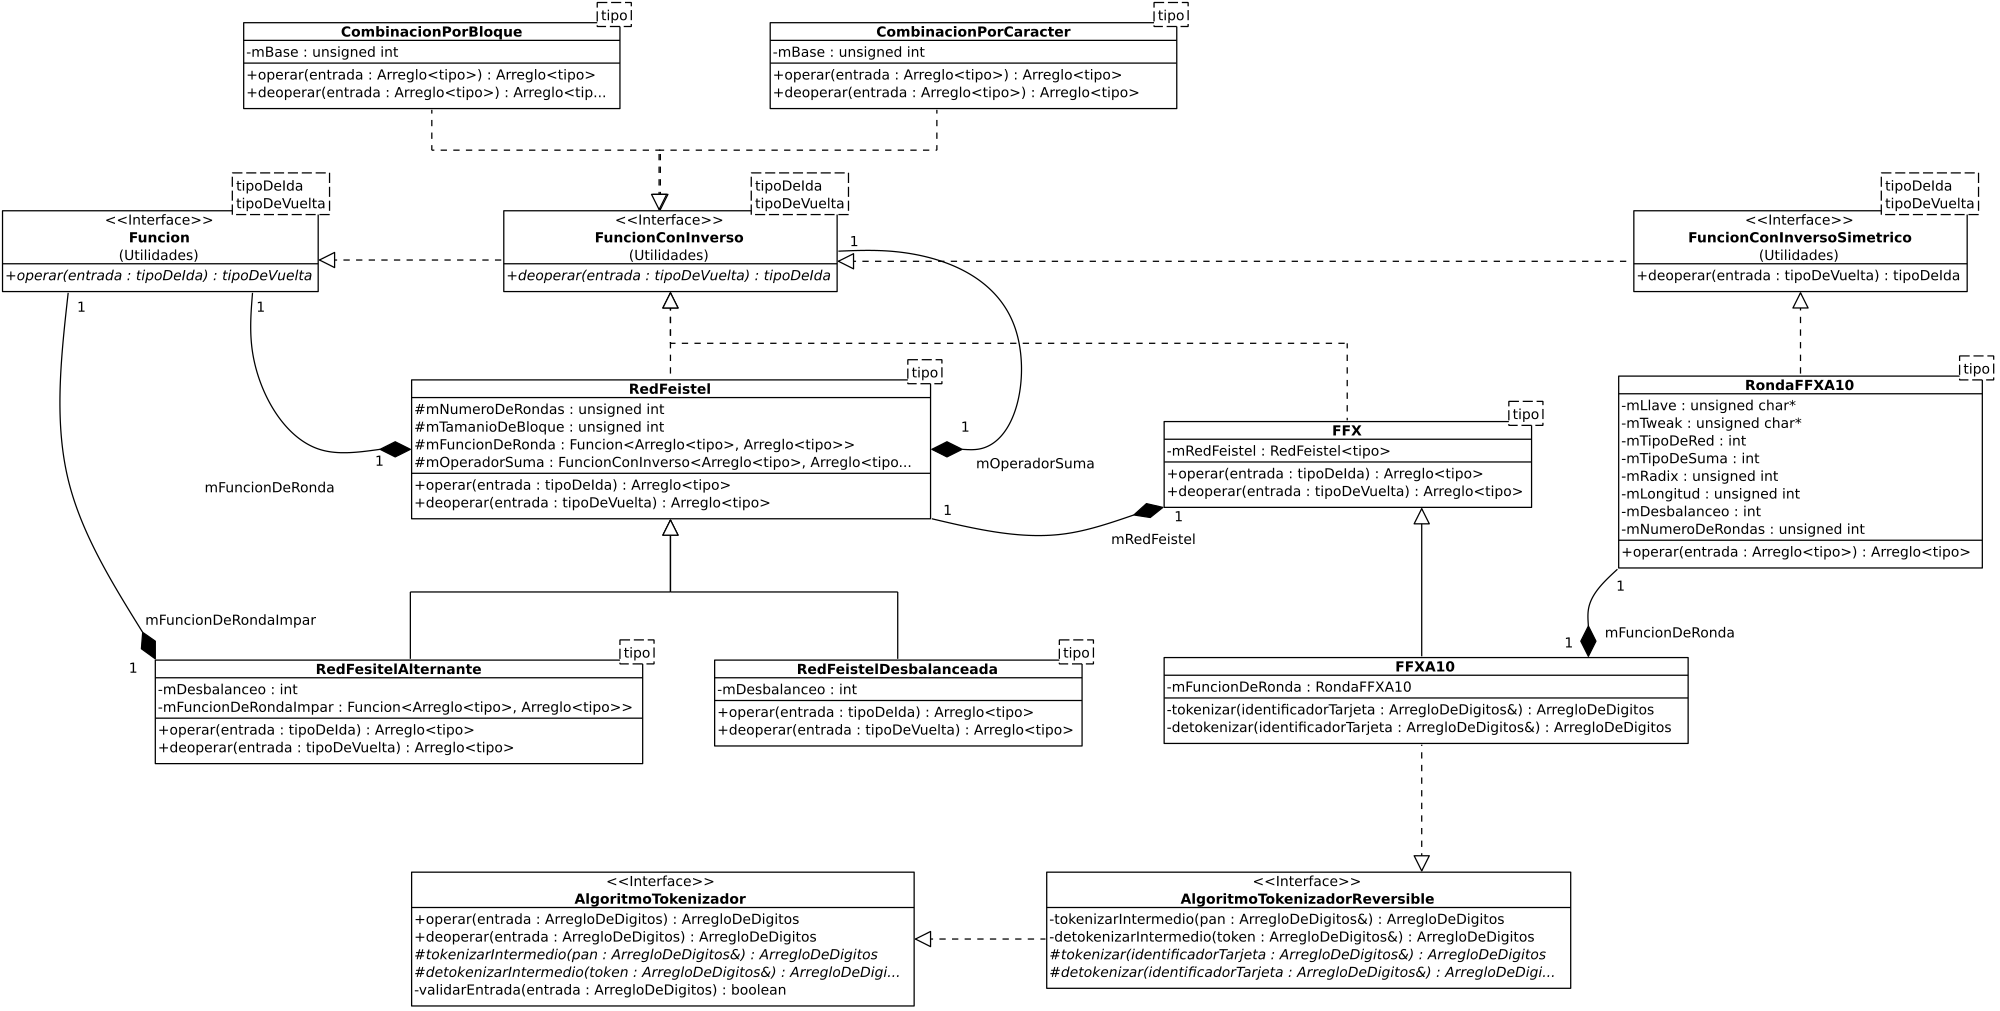
\includegraphics[width=1.0\linewidth]{diagramas/ffx.png}
    \caption{Diagrama de clases de módulo de FFX.}
    \label{clases_ffx}
  \end{center}
\end{sidewaysfigure}
